\section{Introduction} \label{toc:einleitung}

\subsection{Motivation and Introduction} \label{toc:motivation}

The principle of a software-based and decentralized financial system was first described in 2008 with the cryptocurrency \ac{BTC}.
\footcite[Cf.][]{nakamoto2008bitcoin} The basic principle is the provision of a decentralized ledger,
which records all transactions between participants.\footcite[Cf.][]{badertscher2017bitcoin} In order to verify these transactions,
the principle of "mining" was introduced. By making computing power available, the decentralized 
network and thereby secure transactions in the blockchain.\footcite[Cf.][]{kroll2013economics} The voluntary provision of
of computing power is rewarded with the payment of Bitcoins to the owner of the hardware. Initially, it paid out to do Bitcoin
Mining in a private environment with comparatively weak hardware. As interest in Bitcoin increased, so did the number of
of individuals and groups engaged in mining. Due to the resulting increase in the overall computing power of the network, at a certain point
private mining ceased to be profitable, since the maintenance and operating costs of the hardware
exceeded the mining revenue. Subsequently, the business case of "cloud mining" has emerged.\footcite[Cf.][]{taylor2017evolution} This describes
providers that operate data centers specifically for mining cryptocurrencies and sell this service to customers on a pro-rata basis,
who can profit depending on their share of bitcoin payouts from mining.\footcite[Cf.][chap. 3.4.5]{bhaskar2015bitcoin}
To have the profit margin as large as possible for the operating company, there are many factors to consider when building and operating
such data center. The profit margin in operation is basically the difference between the revenue generated by mining
and on the other hand the operating costs and customer payouts. The revenue can be increased by optimizing the efficiency of the hardware.
Operating expenses are largely determined by electricity, spare parts and personnel costs. All these cost items
can be optimized by suitable tools. In addition, after a certain period of time, the start-up investment, such as land, real estate and hardware
must be amortized so that the company is able to make a profit. In such a company (Genesis Group),
which offers cloud mining and owns data centers worldwide, the following thesis takes place. 

One way to visualize and optimize the revenues and expenses of such data centers is to introduce a 
\ac{BI} process. Such are already used to optimize financial data, among other things.\footcite[Cf.][pp. 105]{azma2012business} 
In a \ac{BI} process, data is collected in the first step, subsequently analyzed, and presented to stakeholders at the end,
in order to make decision-making processes transparent and to simplify them.\footcite[Cf.][pp. 1]{loshin2012business} 
In-house data is already collected from \ac{ERP} systems and mining hardware monitoring. 
However, this data is not used further and therefore not submitted to analysis. The analysis and calculation of financial data is
currently supported by a Monte Carlo simulation. However, only idealized data from the data centers are used as starting parameters and 
no real data from the survey are used, since these are not available at this time. In addition, the input parameters are
only estimated. All these components should be combined for a meaningful extension of a \ac{BI} process. The stakeholders of
such a process in this case are the top management and the controlling department, which can use
real data to get a much improved financial picture of a data center. Whether this is reasonably possible 
and how such an implementation can look like, will be clarified in the following of this thesis. The aim is to improve the financially relevant data of a data 
data center and thus to be able to optimize it. 

\subsection{Hypotheses and delimitation of the thesis} \label{toc:hypothesenundabgrenzungderarbeit}

After the thorough analysis of the subject area \ac{BI} and the internal company requirements, the following main hypothesis was 
formulated: 

\textbf{\ac{HT0}: }By introducing a business intelligence process, it is possible to optimize the profitability of a cryptomining
data center. 

In order to be able to work on the main hypothesis better, several sub-hypotheses are formed from this, which divides the main hypothesis into
meaningful subareas. This process has resulted in four sub-hypotheses, which are formulated as follows: 

\textbf{\ac{HT0.1}: }A business intelligence process is used to help management make decisions regarding the
new construction and expansion of mining data centers. 

\textbf{\ac{HT0.2}: }Existing hardware in mining data centers will be optimized by implementing business intelligence. 

\textbf{\ac{HT0.3}: }Business intelligence will improve cash flow evaluation at a mining data center. 

\textbf{\ac{HT0.4}: }Staff planning for a mining data center is optimized through business intelligence processes. 

\ac{HT0.1} deals with the new construction and expansion of data centers. The three other sub-hypotheses are relevant during the operation of a
Cryptomining data center relevant. In the following, all sub-hypotheses are outlined: 

\begin{itemize} 
    \item \textbf{\ac{HT0.1}: }The expansion and new construction of mining data centers is essential for the further development of cloud mining,
    as this will increase the revenue generated by mining. In this context, many influencing factors, such as intrinsic mining
    parameters (Cf. chap. \ref{toc:miningandconsensusalgorithms}), price developments in the \ac{BTC} market, financial drivers, and \acp{KPI}
    (Cf. chap. \ref{toc:key figuresandinfluencingfactors}) of a data center should be taken into account. Due to the complexity and amount of
    different data, \ac{BI} could be a way to support this important strategic process. 
    \item \textbf{\ac{HT0.2}: }The second sub-hypothesis is limited to the technical factors that can contribute to increasing the efficiency of the
    Mining process can contribute. Here, the technical parameters of the hardware are used to identify possible points for improvement
    to identify. This refers to the basics of mining described in chapter \ref{toc:miningandconsensusalgorithms}.
    By applying a \ac{BI} process to the technical parameters, an attempt is made to optimize the efficiency of the existing hardware in this area..
    \item \textbf{\ac{HT0.3}: }In this sub-hypothesis, financial \acp{KPI} are considered. In chapter
    \ref{toc:keyperformanceandinfluencefactors}, these are identified for a mining data center. This hypothesis uses the financial
    metrics and \acp{KPI} that are made visible by implementing a \ac{BI} Process. This allows optimization potentials to be
    found that would be difficult to see without \ac{BI}. The financial optimization ultimately improves the cash flow of a
    data center. 
    \item \textbf{\ac{HT0.4}: }The last sub-hypothesis addresses workforce planning. In a data center, personnel costs are incurred by
    hiring maintenance and local management staff. By analyzing the work involved, such as the
    repair of equipment defects, the staff scheduling of a mining data center can be optimized. This analysis is to be performed by means of a
    \ac{BI} process.
\end{itemize}


All four sub-hypotheses cover the entire spectrum of the main hypothesis with their respective perspectives (technology, finance, personnel, new construction and expansion).

In the following work, some limitations are made. Care is taken to ensure that this does not falsify the research result 
and that the delimitation makes the argumentation more transparent and comprehensible. The following delimitations are made: 

\begin{itemize} 
    \item Only the cryptocurrency Bitcoin is considered. 
    \item As a result, only Bitcoin's \ac{PoW} consensus algorithm is used as the basis for the research. 
    \item There are a variety of different specialized mining hardware on the market. The performance of this hardware is measured by identical 
    parameters. Therefore, one mining hardware model (Antminer S19Pro) is used as an example for the analyses in this work. 
    \item A concrete technical elaboration of a \ac{BI} process as well as its underlying systems is omitted. The focus of this
    focus on the perspective of a \ac{BI} stakeholder and the project management. 
    \item There will be no quantitative or empirical analysis of the hypothesis. The work will rely on qualitative and argumentative 
    deductive analysis as well as a case study.
\end{itemize}

\subsection{Design and structure of the thesis} \label{toc:aufbauundstruktur}

Durch die Formulierung der Haupthypothese ergeben sich die theoretischen Grundlagen, die für die Beantwortung vertieft behandelt werden müssen.
Dies ist im ersten Schritt die Analyse von \ac{BI} Prozessen und deren Grundlagen. In Kapitel \ref{toc:grundlagenbusinessintelligence}
werden die Grundeigenschaften von \ac{BI}, deren betrieblicher Mehrwert und die Voraussetzungen, die ein Unternehmen erfüllen muss, analysiert.
Im nächsten Schritt werden die Grundlagen für das Verständnis von Mining und von Kryptomining Rechenzentren gelegt. Um dies zu erreichen, wird
in Kapitel \ref{toc:grundlagenkryptomining} die Funktionsweise von Blockchains und dem Mining von Kryptowährungen dargelegt. Aufbauend darauf
wird ein Mining Rechenzentrum exemplarisch analysiert, wobei im ersten Schritt der Aufbau und die Funktionsweise und folgend die zentralen
finanziellen Treiber und \acp{KPI} analysiert werden. In Kapitel \ref{toc:ansatzmoeglichkeitenfuerbusinessintelligence} werden die beiden
Grundlagenteile verwendet, um Ansatzpunkte für die Einführung eines \ac{BI} Prozesses zu identifizieren. Dabei wird auch die Prüfung der
Hypothesen vorgenommen. Im letzten Kapitel des Hauptteils wird eine konkrete Implementierung und Modellierung eines \ac{BI} Prozesses
erarbeitet. Damit wird mittels einer Fallstudie überprüft, ob die erarbeiteten Prinzipien aus Kapitel
\ref{toc:ansatzmoeglichkeitenfuerbusinessintelligence} in der Realität umsetzbar sind und die Beantwortung der Hypothesen belastbar ist.
Schlussendlich folgt das Fazit, in dem diese Arbeit kritisch betrachtet wird und mögliche Ansatzpunkte für aufbauende Forschung identifiziert
werden.

\subsection{Relevance in business informatics} \label{toc:relevanzinderwirtschaftinformatik}

Die Wirtschaftsinformatik ist eine interdisziplinäre Wissenschaft, die sich aus den Wirtschaftswissenschaften und der Informatik
zusammensetzt.\footcite[Cf.][p. 5]{mertens2005grundzuge} Einer der langfristigen Ziele der Wirtschaftsinformatik ist die sinnvolle
Automatisierung von Prozessen.\footcite[Cf.][S. 4]{mertens2005grundzuge} Dies bedeutet, dass Aufgaben von Menschen an Anwendungssysteme
übertragen werden, wo dies unter betriebswirtschaftlichen Punkten sinnvoll erscheint.\footcite[Cf.][p. 4]{mertens2005grundzuge}
Business Intelligence ist ein Ansatz, der sowohl wirtschaftliche als auch technische Aspekte in sich birgt und ist daher unmittelbar
in dem Bereich der Wirtschaftsinformatik anzusiedeln.\footcite[Cf.][p. 102]{azma2012business} Dabei ist der wirtschaftliche Teil primär
in dem Bereich der Geschäftsprozesse zu finden. Der technische Teil erstreckt sich in Richtung Big Data und Business Analytics. "The
team needs a champion [...] who understands the business and the technology and is able to translate the business requirements into a
(high-level) BI architecture for a system."\footcite[][p. 27]{yeoh2010critical} Genau für solche Aufgaben kommt der Wirtschaftsinformatik
zentrale Bedeutung zu.

Der Bereich Kryptowährungen ist durch technische und wirtschaftliche Betrachtungsweisen geprägt und ist daher in der Wirtschaftsinformatik
anzusehen, um beide Teilaspekte adäquat würdigen zu können.\footcite[Cf.][]{derks2018chaining} In dieser Arbeit wird geprüft,
ob es möglich ist, mit Hilfe von Business Intelligence das Mining von Kryptowährungen im Umfeld von Rechenzentren optimieren
zu können. Aus den oben genannten Gründen fällt diese Arbeit in den Bereich der Wirtschaftsinformatik. Die Relevanz für
die Wirtschaftsinformatik ergibt sich aus der Kombination der beiden Themengebiete (Business Intelligence und Kryptomining), um eine
finanzielle Optimierung zu erreichen. Es ist dabei unabdingbar sowohl technische als auch betriebswirtschaftliche Aspekte zu analysieren
und einzuordnen, um die Hypothesen der Arbeit zu prüfen und letztendlich verifizieren zu können.

\subsection{Methodology and source selection} \label{toc:methodikundquellenauswahl}

Um die Prüfung der Hypothesen belastbar zu gestalten, wird in diesem Teil die verwendete Methodik, auf die sich diese Arbeit stützt, erläutert.
Des Weiteren ist die Auswahl und der Rechercheprozess für die verwendete Literatur Gegenstand dieses Kapitels. 

Am Anfang der Konzeption dieser Arbeit stand die Literaturrecherche und dadurch eine Identifikation der Forschungslücke, die mit dieser Arbeit
geschlossen werden soll. Die Recherche erfolgt nach den Prinzipien, die von Brocke et al. vorgeschlagen wird.\footcite[Cf.][]{brocke2009reconstructing}
Dabei ist zu beachten, dass die Vorgehensweise nicht in der gesamten Tiefe, die Brocke et al. vorschlagen durchgeführt werden, da der
Fokus dieser Arbeit nicht auf der systematischen Recherche von Literatur liegt. Daher wird folgend der Prozess der Recherche beschrieben. 

\begin{figure}[H] 
    \caption{Procedure in the literature search process} 
    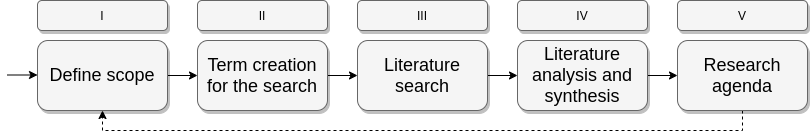
\includegraphics[width=0.9\textwidth]{literaturereview} 
    \label{figure:literaturereview} 
    \\ 
    \cite[Source: Based on][Fig. 3]{brocke2009reconstructing} 
\end{figure} 

Die Recherche teilt sich in einen fünfstufigen Prozess auf, der sequenziell abgearbeitet wird
(Cf. Fig. \ref{figure:literaturereview}):\footcite[Cf.][pp. 2211]{brocke2009reconstructing} 

\begin{enumerate} 
    \item Im ersten Schritt wird der Umfang der Literaturrecherche definiert. Dies geschah in diesem Fall anhand der Themen \ac{BI} und
    des Minings von Kryptowährungen. In Tabelle \ref{tbl:literaturtaxonomie} wird das Ergebnis für den ersten Schritt gezeigt. In
    dieser Tabelle wird eine Literaturtaxonomie nach Cooper vorgenommen.\footcite[Cf.][p. 2212]{brocke2009reconstructing}\footcite[Cf.][]{cooper1988organizing} 
    \item Folgend werden die Suchbegriffe für die Literatursuche gebildet. Allerdings wird dieser Schritt kontinuierlich abhängig von
    den Ergebnissen angepasst. Es wird nach den Abkürzungen als auch nach deutschen und englischen Begriffen gesucht. Die verwendeten 
    Suchabfragen sind in Tabelle \ref{tbl:suchprozessergebnis} aufgelistet.\footcite[Cf.][pp. 2211]{brocke2009reconstructing} 
    \item In diesem Schritt wird die eigentliche Literatur gesucht. Als Suchplattformen werden Google
    Scholar\footnote{https://scholar.google.com}, EBSCO\footnote{https://www.ebsco.com}, Wiso\footnote{https://www.wiso-net.de}, 
    SpringerLink\footnote{https://link.springer.com} und IEEExplore\footnote{https://ieeexplore.ieee.org} verwendet. Es wird darauf
    geachtet, dass es sich nach Möglichkeit immer um peer-reviewed Veröffentlichungen handelt, die in wissenschaftlichen Journalen
    erschienen sind. Es werden zum Teil auch Bücher und Online Quellen verwendet. Diese werden nicht als Grundlage für die zentrale
    Argumentation der Arbeit verwendet, da diese Bücher nicht als wissenschaftliche Literatur angesehen werden können. Das Ergebnis der
    Recherche findet sich in Tabelle \ref{tbl:suchprozessergebnis}. 
    \item Es wird nun die Literatur analysiert und gegliedert. Dazu werden Themenbereiche definiert, denen die gefundene Literatur
    zugewiesen wird. Das Ergebnis davon findet sich in Tabelle \ref{tbl:konzeptmatrix}.\footcite[Cf.][p. 2214]{brocke2009reconstructing}\footcite[Cf.][]{webster2002analyzing}  
    \item Im letzten Schritt wird die Forschungsagenda basierend auf der Forschungslücke erarbeitet. Diese ist bei dieser Arbeit in
    der Anwendung von \ac{BI} im Bereich Mining von Kryptowährungen. Es gibt zahlreiche Veröffentlichungen über die Optimierung von Mining
    Prozessen.\footcite[Cf.][]{han2019demystifying}\footcite[Cf.][]{courtois2014optimizing} Zudem existieren Veröffentlichungen im
    Bereich Mining Hardware sowie Mining und Blockchains in der Cloud.\footcite[Cf.][]{taylor2017evolution}\footcite[Cf.][]{gai2020blockchain} 
    Weiterhin sind Forschungspaper im Bereich Aufbau von Mining Rechenzentren zu finden. Dabei wird sich eher auf den Aufbau von
    \ac{ASIC} basierten Rechenzentren fokussiert, welches für Bitcoin passend ist.\footcite[Cf.][]{li2019blockchain}\footcite[Cf.][]{xie2018extreme}
    Die betrachteten Rechenzentren betreiben Mining ausschließlich durch \ac{ASIC} basierte Hardware. Dementsprechend gibt es auf der
    Seite des Kryptominings zahlreiche Veröffentlichungen über das Thema Optimierung des Minings. Wenn nach einer Verbindung von
    Kryptomining und \ac{BI} gesucht wird, ist jedoch die Auswahl deutlich kleiner. Es gibt Literatur, die sich mit der Kombination von
    Kryptowährungen und \ac{BI} beschäftigt, die allerdings eher im Bereich Preis- und Kursentwicklungen zu finden
    ist.\footcite[Cf.][]{botocs2017bitcoin} Im Bereich der Optimierung von Mining Infrastrukturen mittels \ac{BI} ist nichts zu finden.
    Dies liegt zum einen an wenigen großen Unternehmen, die Bitcoin Mining betreiben und die deren Optimierungen und Effizienzsteigerungen
    aufgrund der harten Konkurrenz nicht veröffentlichen.\footcite[Cf.][]{btccom2021miner} Zum anderen ist der Kryptowährungshype der
    letzten Jahre eher im Bereich des Investments und der Weiterentwicklung der Blockchain Technologie und weniger im Bereich
    Mining.\footcite[Cf.][]{friedlmaier2018disrupting} 
\end{enumerate} 

\begin{figure}[H]
    \caption{Method profile of business informatics}
    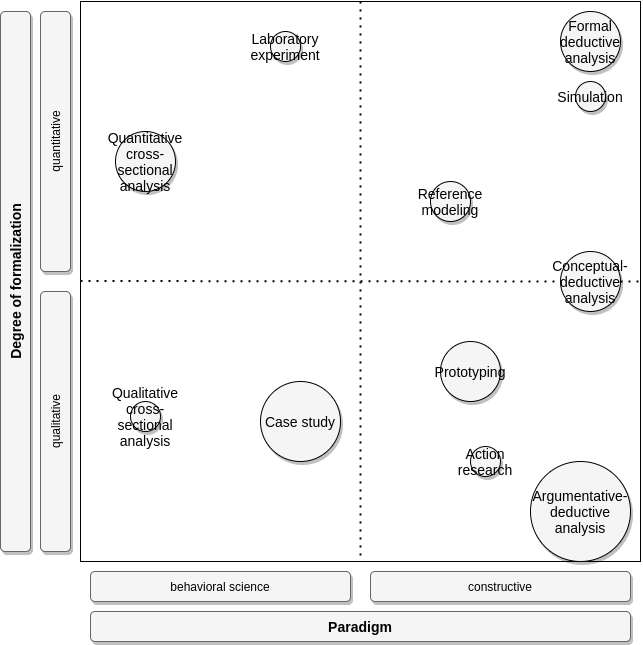
\includegraphics[width=0.7\textwidth]{methodenprofilwi}
    \label{figure:methodenprofilwi}
    \\
    \cite[Source: Based on][Fig. 3]{wilde2007forschungsmethoden}
\end{figure}

Für die Evaluation der richtigen Methodik, um die Hypothesen dieser Arbeit zu prüfen, werden die möglichen Methodiken in der
Wirtschaftsinformatik allgemein und im Bereich \ac{BI} speziell
analysiert.\footcite[Cf.][]{wilde2007forschungsmethoden}\footcite[Cf.][]{wilde2006methodenspektrum}\footcite[Cf.][]{jourdan2008business} 
Dabei ist feststellbar, dass sowohl die argumentative-deduktive Analyse als auch die Fallstudie die ersten beiden Plätze bei der
Verwendung belegen.\footcite[Cf.][Fig. 2]{wilde2007forschungsmethoden} Auch werden bei der Mehrzahl der Veröffentlichungen im Bereich
\ac{BI} qualitative Methoden verwendet.

Um die Hypothesen prüfen zu können werden folgende qualitative Methodiken verwendet: 

\begin{itemize}
    \item \textbf{Argumentativ-deduktive Analyse: }Dabei handelt es sich um eine konstruktionswissenschaftliche Methode, die primär auf
    der Anwendung einer logischen Argumentationskette aufbaut.\footcite[Cf.][Tbl. 1]{wilde2007forschungsmethoden} Diese wird in Kapitel
    \ref{toc:ansatzmoeglichkeitenfuerbusinessintelligence} angewendet und basiert auf den Grundlagen der beiden vorangegangenen Kapiteln.
    Es findet mittels einer argumentativen-deduktiven Analyse die erste Prüfung der Hypothesen statt. 
    \item \textbf{Fallstudie: }In Kapitel \ref{toc:planungeinesbiprozessesfuereinminingrechenzentrum} wird basierend auf den theoretischen
    Ergebnissen eine Fallstudie konzipiert. Diese wird qualitativer Natur sein und stellt eine weitere Prüfung der Hypothesen dar. Im
    Unterschied zur argumentativen-deduktiven Analyse wird in der Fallstudie die Prüfung der Hypothesen in einem realen Umfeld vorgenommen.
    Daher ist eine Fallstudie nicht zu den konstruktionswissenschaftlichen Methoden, sondern zu den verhaltenswissenschaftlichen Methoden
    (Cf. Fig. \ref{figure:methodenprofilwi}) zu zählen. Bei der Konzeption der Fallstudie wird nach der Veröffentlichung von Göthlich
    vorgegangen.\footcite[Cf.][]{gothlich2003fallstudien} Die Stakeholderanalyse wird anhand der Veröffentlichung von Simmers
    vorgenommen.\footcite[Cf.][]{simmers2004stakeholder} Die Analyse einer Einführung wird primär durch die Texte von Loshin und
    Boyer et al. geprüft.\footcite[Cf.][]{loshin2012business}\footcite[Cf.][]{boyer2010business}
\end{itemize} 

Durch die Prüfung der Hypothesen mittels zweier unabhängiger Methodiken wird versucht, dass die Hypothesen aus verschiedenen Standpunkten analysiert
werden und dadurch das Ergebnis dieser Arbeit belastbar ist.